\section{Beat Box}
Along with melody and harmony, rhythm is one of the most important components of music. The exhibit ``Beat Box'' explores various ways to create and analyze rhythms by mathematical methods.

\subsection{Fibonacci Rhythm / Hemachendra (Fibonacci) numbers and 2-1 rhythms}
It only seldom happens in science that important concepts are named after the person who dealt with them first. This is also the case for the famous Fibonacci numbers. Fibonacci mentioned them in the context of a calculation exercise in his book Liber Abaci published in 1202. As a matter of fact already much earlier in 1050 these numbers were studied by the Indian scholar Hemachendra in a very interesting context related to rhythm.

\begin{wrapfigure}[24]{l}{0.4\textwidth}
\centering
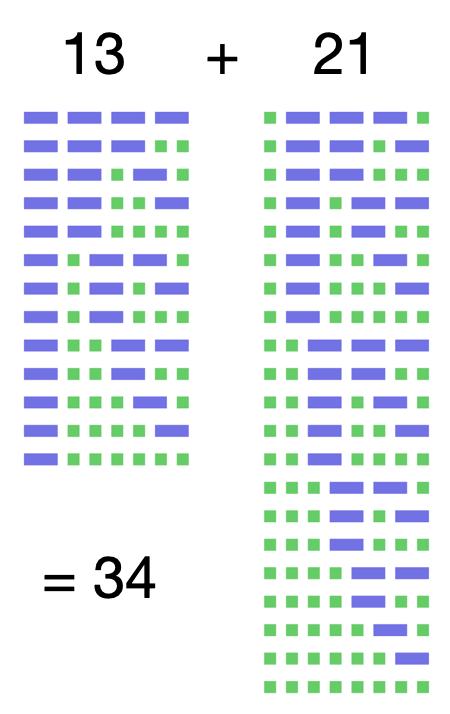
\includegraphics[width=0.4\textwidth]{BeatBox_1}
\caption*{Fibonacci rhythm}
\end{wrapfigure}
Assume you want to fill a rhythm of n beats with patterns of either length 1 or of length 2. For instance an 8-beat rhythm could be filled by 1-1-1-1-1-1-1-1 or 2-2-2-2 or more complicated patterns like 2-1-2-1-2 or 2-1-2-2-1. How many possibilities are there? Such questions arise both in poetry when talking about verses and syllables, or in music when talking about rhythms built from quarters and halves. It turns out that the number of actual possibilities is a Fibonacci (or better Hemachendra ) number. A number from the sequence
\begin{center}
1, 1, 2, 3, 5, 8, 13, 21, 34, 55, 89, 144,...
\end{center}
where (after starting with 1, 1) each number is the sum of the preceding two. In fact there are exactly 34 ways to fill an eight beat pattern with 1s and 2s.

\paragraph{The Music:}
To avoid repetitive patterns in music it is sometimes very good to be aware of all possibilities that satisfy a given requirement. The question of filling in beats with longs and shorts for instance has nice applications in the art of tabla playing. Here often the shorts and longs are not literally one note but fixed drumming patterns that fill either one or two beats. Using only two fixed patterns but being flexible with the macro rhythmic level of how to combine them creates a stylistic coherence while at the same time it creates richness.

\paragraph{The Math:}
Why do Fibonacci numbers pop up in this context? Let us see how we can reduce the problem of filling 8 beats to the problems of filling 6 and 7 beats. Each eight beat rhythm either starts with a short or with a long note. If it starts with a long note there are as many ways to complete this as there are 7 beat patterns. If we start with a long  note then we have 6 beats to fill and there are as many possibilities as there are for 6 beats. Hence the number of 8 beat patterns equals the sum of the number of 7 beat and 6 beat patterns. Et voilà... the Fibonacci recursion.

\paragraph{The Exhibit:} The exhibit is mainly an automatic tabla rhythm machine based on the above observations. Listen and enjoy! The sound samples for the fast Rhythm were, by the way, taken from a talk of Manjul Bhargava, a Fields Medalist, who also gave very inspiring talks on that topic, where he himself plays the tabla.

\subsection{Clapping / Steve Reich's Clapping Music}
Want a challenge? Here it is! Try to clap along with one of the two voices in our Clapping exhibit. Or even better, find a partner and together clap both voices. For every position of the green point in the exhibit the challenge is different.

The piece you hear in the exhibit is an amazing example of how a simple idea can create interesting and complex musical patterns. Inspired by the clapping of Flamenco dancers, Steve Reich composed this amazing little piece of music. It consists of a simple 12-beat clapping pattern:

\begin{figure}[h]
\centering
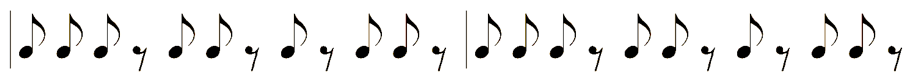
\includegraphics[width=0.9\textwidth]{BeatBox_2}
\caption*{3 claps - pause - 2 claps - pause - 1 clap - pause - 2 claps - pause ... repeat}
\end{figure}


The complexity is achieved by playing exactly the same rhythm with two players but shifting the beginning of the second player by n-beats for a chosen number n=0 to n=11. There are twelve possible such shifts each generating a different rhythm. Can you clap all of them with your partner?

\paragraph{The Music:}
A Minimal Music (mainly composed by Steve Reich) attempts to create interesting music by minimalistic progression of score. Shifting a rhythmical pattern by just one beat might be considered as a typical stylistic element of Minimal Music. In fact the clapping piece needs a tremendous concentration as soon as both parts are played together. Hence although it is minimal it is by no means easy.

\paragraph{The Math:} How many rhythmical patterns are suitable for creating a piece like Clapping Music. Let's stick to a 12 beat sequence. First of all there are altogether $2^{12} = 4096$ possibilities to have either clap or pause at one beat.

We might require that the pattern itself has no repetitions since this would cause identical music under more than one shift. This kills 76 of the patterns. Of the remaining 4020 patterns we only need one shifted version of each. This dived the total number by 12 and leaves us with only 335 patterns.

\begin{wrapfigure}[13]{l}{0.33\textwidth}
\centering
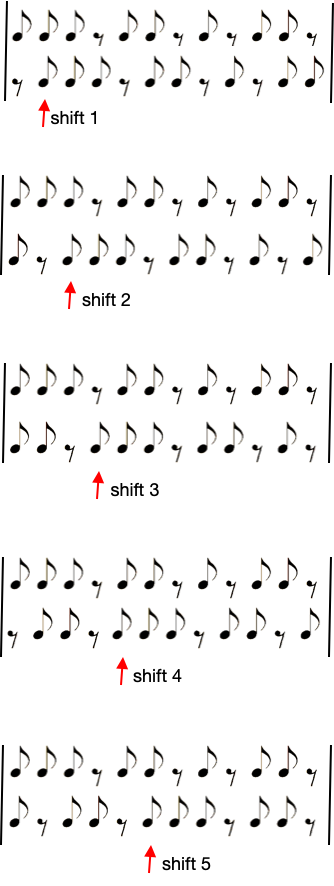
\includegraphics[width=0.33\textwidth]{BeatBox_3}
\end{wrapfigure}

Most of them would sound pretty boring since there are either too many or too few claps played. Restricting to patterns with at least 4 and at most 8 claps leaves us with 287 possibilities. Narrowing down further and requiring that like in Reichs piece no consecutive pauses occur leaves us with no more than eleven patterns (shown below). Reich's choice (marked in red) is one of only two without repeating the number of claps between two pauses.

% \begin{figure}[h]
% \centering
% 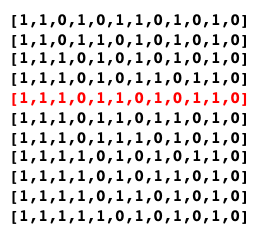
\includegraphics[width=0.4\textwidth]{BeatBox_4}
% \end{figure}

\hfill \makebox[0.6\textwidth][c]{
\ttfamily \bfseries
\begin{tabular}{c}
(1,1,0,1,0,1,1,0,1,0,1,0) \\
(1,1,0,1,1,0,1,0,1,0,1,0) \\
(1,1,1,0,1,0,1,0,1,0,1,0) \\
(1,1,1,0,1,0,1,1,0,1,1,0) \\
\color{red}(1,1,1,0,1,1,0,1,0,1,1,0)\color{black} \\
(1,1,1,0,1,1,0,1,1,0,1,0) \\
(1,1,1,0,1,1,1,0,1,0,1,0) \\
(1,1,1,1,0,1,0,1,0,1,1,0) \\
(1,1,1,1,0,1,0,1,1,0,1,0) \\
(1,1,1,1,0,1,1,0,1,0,1,0) \\
(1,1,1,1,1,0,1,0,1,0,1,0) \\
\end{tabular}
}
\paragraph{The Exhibit:}
Go and clap along. Try to start slowly and increase your speed. Select the different shifts by moving the green point on the circle.

\vspace{12ex}

\subsection{Sequencer}
Have you ever stepped in to a printing hall of a big newspaper?
Where the machines spin round and round and create a sound pattern with each rotation. Or just listened to a sewing machine? Whenever some mechanical process produces a repeating pattern our brain is trained to search for structure in it. Forming rhythm. Forming music. The beat machine in our exhibition is a sequencer that lets you experiment with cyclic patterns. Play and explore.

\paragraph{The Exhibit:}
Perhaps a little usage description is useful here. Consider the four big wheels as turntables equipped with bars. Whenever the bars hit an instrument it creates a sound. The instruments are resembled by the five small colored points in the central area. You can move them around freely. If they get hit they make a sound. Which instrument is resembled by each point can be chosen by the colored sliders at the far right. The further out an instrument is on a wheel, the louder it is played.

When the machine is at rest, the number of bars on each disk can be changed by moving the sliders. By this, it is possible to create very uneven but still cyclic repetition patterns. For instance you can set one of the disks to 8 bars per turn, the other to 11 and the other two to 15. This sounds wild but still very rhythmic. As a matter of fact, African music cultures are by far more used to such uneven rhythm distributions than Western ones.

\begin{figure}[h]
\centering
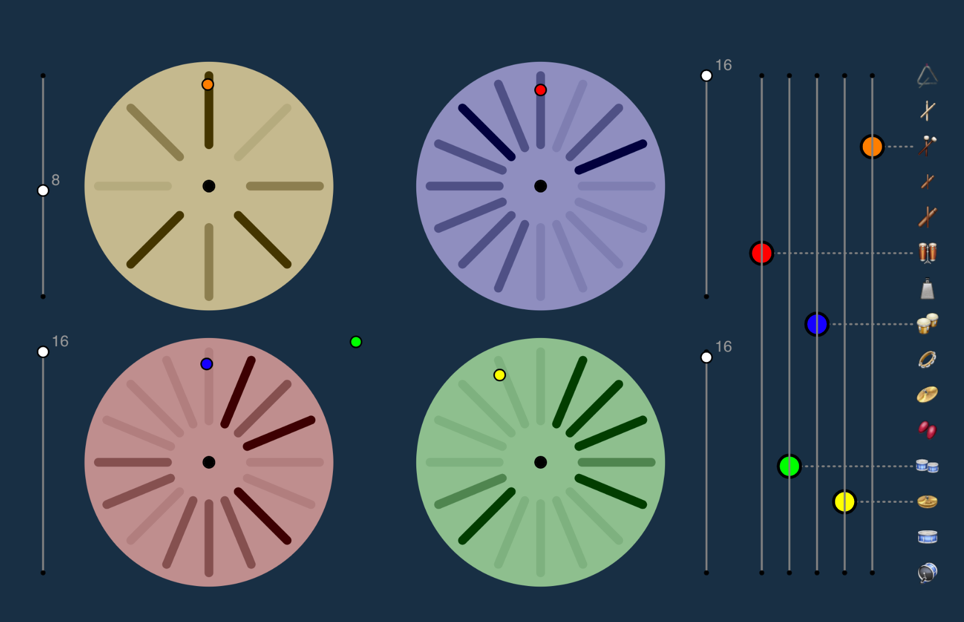
\includegraphics[width=0.9\textwidth]{BeatBox_5}
\end{figure}

In the rest state you can also click on the bars on the disk and alter them between three states, loud-medium-off. By this you can create a great variety of known and of totally new rhythms.


\subsection{n over m Rhythms}
We are very much used to clap simple regular rhythms like a two-step march 1-2-1-2-1-2 or a waltz in a three fold pattern 1-2-3-1-2-3. It is perhaps one of the first exercises when learning a percussion instrument to be able to perform these kinds of rhythms. But things become really difficult if we want to clap two rhythms simultaneously. Combining a regular rhythm with n beats in a bar with another rhythm, that has m beats in the same time is called an n over m rhythm. The speed ratio between the two rhythms is then n/m. The picture below illustrates a 2 over 3 rhythm. In each bar the top voice has exactly two evenly distributed notes while the lower voice has three evenly distributed notes.

\paragraph{The Math:}
Perhaps the easiest way to learn simple n over m rhythms is to merge them into a common framework of constant ticks fine enough to incorporate both rhythms. Mathematically this asks for the least common multiple of the two numbers n and m. Thus a 2 over 3 rhythm can be embedded in a regular rhythm of 6 ticks, a 3 over 4 rhythm can be embedded in 12 ticks and a 7 over 5 rhythm can be embedded into a rhythm with 35 ticks. If one counts the ticks by starting from zero the  m-beat rhythm is played on the multiples of n and the n-beat rhythm is played on the multiples of m.

\begin{figure}[h]
\centering
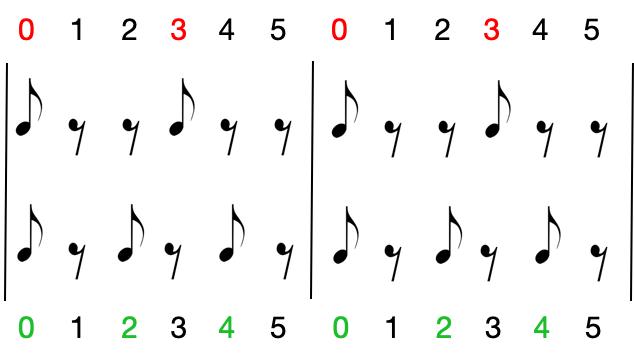
\includegraphics[width=0.7\textwidth]{BeatBox_6}
\end{figure}

\paragraph{The Music:} Playing the n over m rhythm in the above way is a good way to learn it. However it has one big disadvantage. One does not ``feel'' the rhythm as being composed from two distinct regular ones.

Here is a ``pro tip'' for learning these rhythms. First learn to clap them with two hands by using the above method (it will take a while). After feeling secure in clapping these rhythms play them and ``split your mind'' and focus to only one hand and what it does. And then switch the mind between the two hands. At some point you will be able to feel both rhythms independently and simultaneously in your mind.

\begin{figure}[h]
\centering
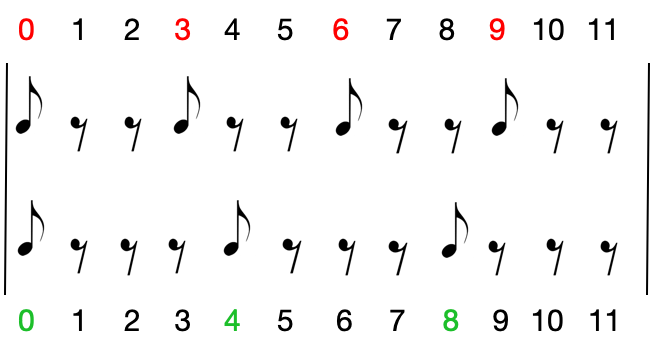
\includegraphics[width=0.7\textwidth]{BeatBox_7}
\end{figure}

\paragraph{The Exhibit:} The exhibit is a clap along exhibit. You can hear and experience n over m rhythms and you can also try to learn clapping them. It might take a little practice but once you get it you won't un-learn.


\subsection{Grid Rhythms}
Can you hear the rhythm of a regular ornamental drawing? Have you ever rushed with a trolley over a regular pavement busy to get your train or airplane? Did you listen to the sound it created? In fact already for the simplest geometric patterns (like a square grid) moving a point over it in constant speed creates interesting rhythmical patterns. If you associate different voices to the horizontal and vertical lines of a grid then moving a point in any direction with constant speed over the grid creates a regular rhythmic pattern in each voice. However the two patterns have different speed and are shifted in phase, leaving lots of space for musical experience.

\paragraph{The Music:} Getting inspirations for interesting musical patterns is an important part of the work of creative musicians. Those inspirations can come from very different sources.

We strongly recommend to listen to the YouTube Video ``Stoiber on Drums'' in which a percussionist performs along with Edmund Stoibers speech about a fast train connection from Munich Center to the Airport trying to hit an instrument every time there is a syllable in the speech.

\begin{figure}[h]
\centering
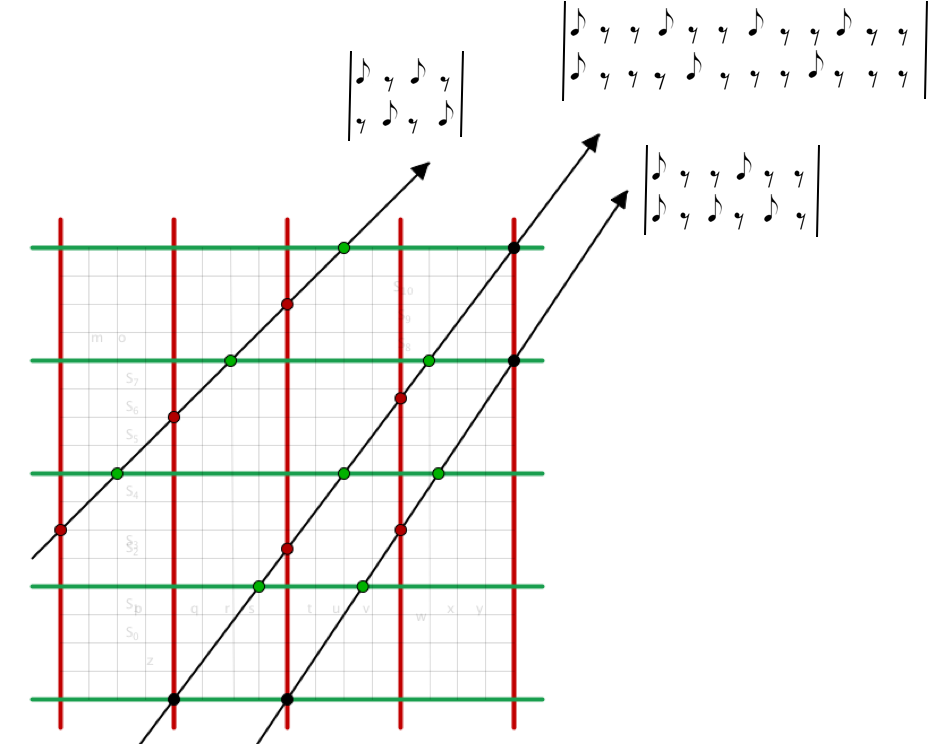
\includegraphics[width=0.7\textwidth]{BeatBox_8}
\end{figure}

\paragraph{The Math:} The square grid creates an overlay of two regular beat patterns. As a matter of fact except for the regularity of each pattern everything else is free in this context: both speeds and the phase between them. The examples in the figure show a few instances, among them a 2 over 3 and a 3 over 4 rhythm. If the slope of the line is irrational (not a fraction) then the rhythmic pattern generated will even never repeat.

\paragraph{The Exhibit:} By adjusting the slope of the movement you can experience all possibilities that are accessible through that approach of rhythm generation. You can adjust the direction of the grid motion. Pressing one of the synchronize buttons sets the grid to the indicated position with respect to the measuring point. This allows you to get a bit more control over the rhythm.


\subsection{Euclidean Rhythm / Line Step Rhythms}
How to distribute 3 drum hits in a measure of 8 beats? And what does this have to do with low resolution computer screens? Here is a nice connection. Imagine you want to draw a line with slope 3/8 on a low resolution grid by a pixelized line. The picture below indicates the line as a sequence of highlighted pixels. The steps in that image form a regular and rhythmic pattern. The slope of 3/8 implies that while you go 8 units to the right you must go also 3 units up. Thus the pattern repeats after 8 steps. If you hit a drum every time you step up, you get a nice pattern of 3 hits distributed over 8 beats.

\begin{figure}[h]
\centering
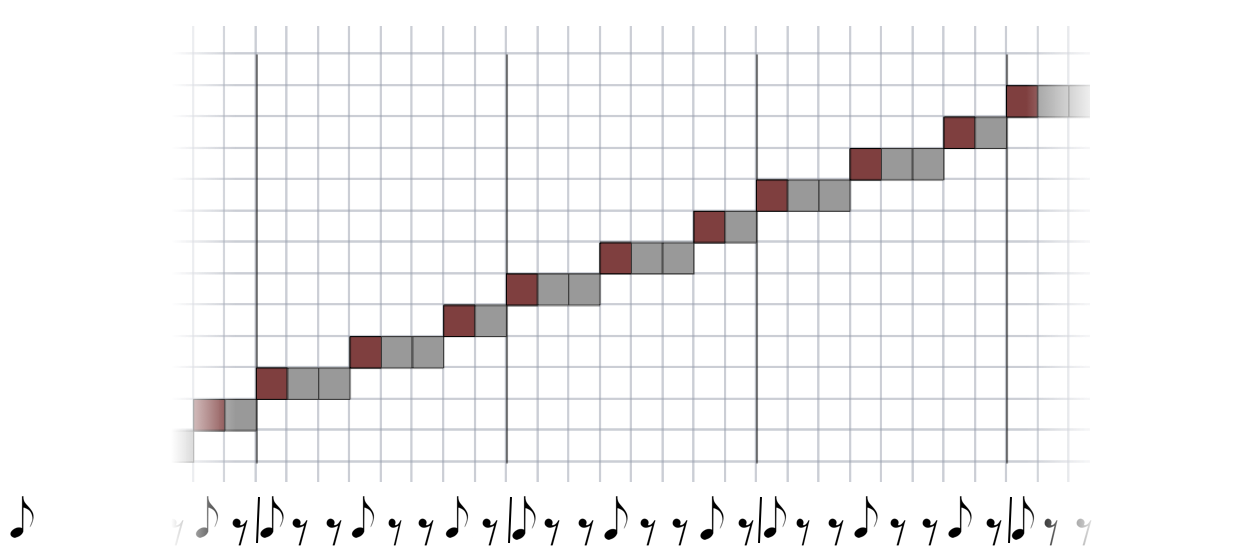
\includegraphics[width=0.7\textwidth]{BeatBox_9}
\end{figure}

\paragraph{The Math:} This generation method for a rhythm has a remarkable property. It distributes the 3 hits as equal as possible among the 8 beats.
The reason for that is that the pixelized drawing of the line approximates the line as good as possible.
\begin{wrapfigure}[13]{r}{0.4\textwidth}
\centering
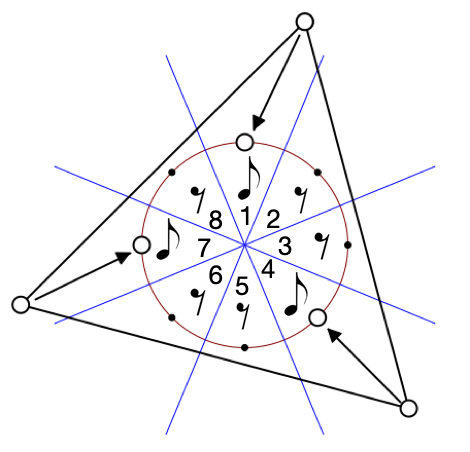
\includegraphics[width=0.39\textwidth]{BeatBox_10}
\end{wrapfigure}
 Another way to think about this generation method is to consider an equilateral triangle and then to choose points from an octagon with same centre that are as close as possible to the corners of the triangle. Clearly the method can easily be generalized to any number of hits and beats.

\paragraph{The Music:} The equal distribution indicated by this method creates very interesting rhythms. As a matter of fact they can be found across all different cultures and styles from Balkan folklore, via Latin American and Japanese rhythms, to Dave Brubeck's Take Five and Unsquare dance.

\paragraph{The Exhibit:} In the exhibit you can create two such rhythms in parallel and vary the numbers that generate the rhythms. It is a great device to create and exercise quite complicated and elaborate rhythm patterns.




\begin{sectcredits}
\item[Author of this exhibit:] Jürgen Richter-Gebert (Technical University of Munich).

\item[Acknowledgements:] Patrick Wilson and Aaron Montag (Sound Engine). Based on CindyJS.org.

\item[Text:] Jürgen Richter-Gebert (TU Munich).
\end{sectcredits}
